% PACKAGES LOADED-------------------------------
\documentclass[10pt,letterpapter]{article}
\usepackage[left = 1in, top = 1in, bottom = 1in, right=1in]{geometry}
\usepackage{csquotes}
\usepackage{graphicx}
\usepackage{amssymb}

%BEGIN DOCUMENT-----------------------------------------
\begin{document}

%TITLE, AUTHOR-------------------------------
\title{ \textbf{Airbnb Capstone: Super Host Analysis}}
\author{Justin Malunay}
\maketitle

%BEGIN ABSTRACT----------------------------------------
\begin{abstract}
This report discusses the significance of Airbnb's Super Host Program. Based on Airbnb's open data, I was able to predict the amount of super hosts in 2015 - 2016 for the following year, 2016 - 2017. This report contains my analysis and explanation of my processes. This is a project I've worked on during the last couple of weeks of the Data Science Immersive Program at General Assembly in San Francisco, CA.  
\end{abstract}

%BEGIN INTRO PARAGRAPH--------------------------------
\section{Introduction}
%\setlength\parindent{24pt}
\begin{paragraph}
\indent
Airbnb is a community marketplace for people to rent their homes or private rooms to guests from all over the world sharing the best experiences and vice versa. It provides a service without having the hassle to find a hotel and gives a variety of rooms or entire homes. Airbnb was first established in 2008, and a total of about:
\begin{itemize}
	\item 60,000,000+ Guests
	\item 40,000+ Cities
	\item 1,400+ Castles
	\item 191+ Countries
\end{itemize}
\end{paragraph}
\indent
By the end of 2008, Airbnb generated about 1 million dollars in revenue. 

\begin{paragraph}
\indent 
The data collected came from Airbnb's Open Database. It contains 35 major locations, but I focused on San Francisco, CA alone. I used the listings csv file which consisted of hosts names, location, neighborhood, price per unit, type of room, and more. The most interesting feature is the term,  \textbf{super hosts}. 
\\ \\
\textbf{Note:} The data are only listings,  \textbf{NOT} bookings. This is solely for the privacy and safety purposes. 
\end{paragraph}

%OBJECTIVE-------------------------------------- 
\section{Objective}

%PROBLEM STATEMENT
\textbf{Problem Statement:}
\begin{paragraph}
\indent 
What are super hosts? I will determine what a super host is based on the data and simple research. Using data analysis, machine learning, and various algorithms I will predict the amount of future super hosts. Overall, I will find the purpose of super hosts and how they benefit not only Airbnb's market, but the host themselves.
\\ \\
%HYPOTHESIS
\textbf{Hypothesis:}
\\ \\
\indent \indent I believe Super Hosts are they key to generating the most revenue for Airbnb. In addition to showing the most hospitality for guest, I believe the type of room, price, and neighborhood will determine who will be next future hosts.
\end{paragraph}

%RESEARCH SUMMARY 
\textbf{Research Summary:}
\\ \\
\textbf{Super Hosts:} Hosts that provide the best experience for guests, and also achieve the following in the \indent \indent \indent \indent \space \space \space \space current \textbf{year}:

\begin{itemize}
	\item Housed or hosted a total of 10 trips or bookings from guests
	\item Maintain a minimum of 90\% response rate to his or her guests. The host must notify any requests given by 24 hours
	\item Must have at least 80\% of reviews to be 5-stars
	\item Complete a reservation with \textbf{NO} cancellations
\end{itemize}

All requirements must be met before the current year ends if a host wants to qualify as a \textbf{super host}.

%EXPERIMENTAL PROCEDURE---------------------------------------
\section{Experimental Procedure}

%STEP 1 
\textbf{Step 1: Cleaning the Data} 
\begin{paragraph}
\indent
Some rudimentary cleaning was needed. For my \enquote{price} and \enquote{percentage} columns, they were in object types. I used a list comprehension to iterate through the columns and convert them to string. Then, I created another list comprehension to replace \enquote{\$} with a blank space. I repeated this step to replace any commas (,) as well. The purpose for this is for further summary statistics and data analysis. This is necessary for using pandas and numpy functions. 
\\ \\ 
\indent \indent
The other variable I changed was the \textbf{super host}. The values of this columns consisted of \enquote{t} and \enquote{f}, which represented \textbf{True} and \textbf{False}, respectively. For this part I used binary where 1 equals \textbf{True} and 0 equals \textbf{False}. (1 represents the super host, 0 represents a normal or non super host). The purpose for this step is for further classification predictions. 

\end{paragraph}

%STEP 2
\indent \\
\textbf{Step 2: Exploratory Data Analysis} 
\begin{paragraph}
\indent
After all the data cleaning, I calculated some basic summary statistics. There are a total of 4,647 hosts. 723 hosts are super hosts (16.0\%) and the remaining 3924 hosts are normal or non super hosts (84.0\%).  By taking the total sum of prices per month, we are able to see a trend from January to December. There is a steady increase until it hits November - range 27 million to 36 million dollars. However, both months November and December are significantly lower, 17 million and 23 million dollars respectively. We can interpret that listings in November and December were limited due to the holiday seasons of Thanksgiving and Christmas. 
\\ \\
\indent \indent
Next, I grouped the total listings and average price per neighborhood for both non super hosts and super hosts. For non super hosts, the top 5 neighborhoods with most listings are Mission District (578 listings), Soma (309 listings), Richmond District (218 listings), Western Addition / NOPA (197 listings), and Noe Valley (181 listings). The top 5 average priced neighborhoods are Forest Hill (\$402.11), Cole Valley (\$397.42), Sea Cliff (\$350.00), Financial District (\$348.80), and Mission Bay (\$308.33). In comparison to the super hosts, the top 5 districts with the most listings are Mission District (100 listings), Castro (64 listings), Western Addition / NOPA (51 listings), Bernal Heights (46 listings), Richmond District (42 listings). And as for the top 5 average priced neighborhoods are Pacific Heights (\$389.00), South Beach (\$385.00), Cow Hollow (\$362.50), Marina (\$317.88), and West Portal (\$288.00). 

\end{paragraph}

%STEP 3
\indent \\
\textbf{Step 3: Algorithms / Methods} 
\begin{paragraph}
\indent
In order to proceed with further analysis, I needed to find some sort of correlation between the variables present. In addition, after cleaning there were still categorical variables that needed actual values to be substituted. There were several columns which had True and False values, so I used binary values where the True values equal to 1 and False values equal to 0. I them used numpy to correlate the data and created a heat map using seaborn to visually see a correlation of the features. Another method I used came from the Decision Tree Classifier algorithm.
\\ \\ 
\indent \indent In this case, I imported patsy to convert these categorical variables to numerical variables. The Decision Tree Classifier allows me to pull out the most important features. I ranked them starting with the highest coefficient value. They are as followed: reviews per month (0.27), reviews score rating (0.19), price (0.12), availability 365 (0.10), host acceptance rate (0.07), host response rate (0.06), and host total listings (0.22). From previous research, we know that the reviews score and host response rate are key features for being a \textbf{super host}. This validates my findings, so i proceed with machine learning.
\\

\indent \indent
First of all, my baseline accuracy came out to 15\%. The first model I ran was k Nearest Neighbors (kNN). This algorithm classifies each data point based on the other data points which are closest in distance. By performing a grid search, I was able to find the best parameters for kNN and one of them was the classifying data points (20 neighbors). My scores for kNN:
%ADD SCREEN SHOTS HERE!!!!-------------------------------------------
\\ \\
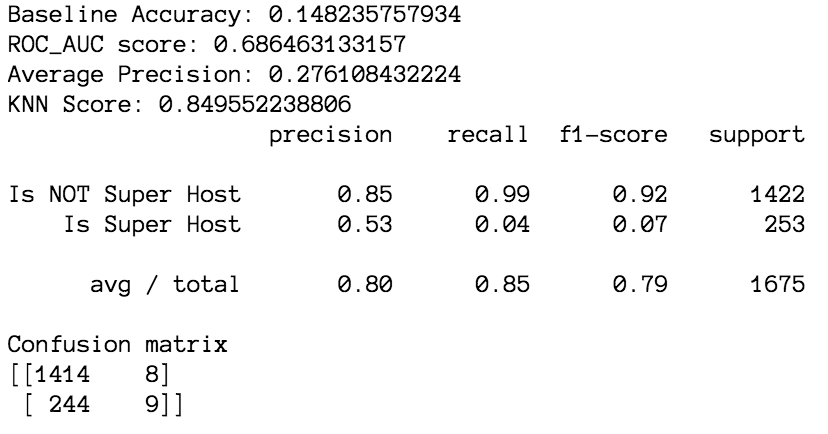
\includegraphics[scale=0.65]{knnscores.png} \\
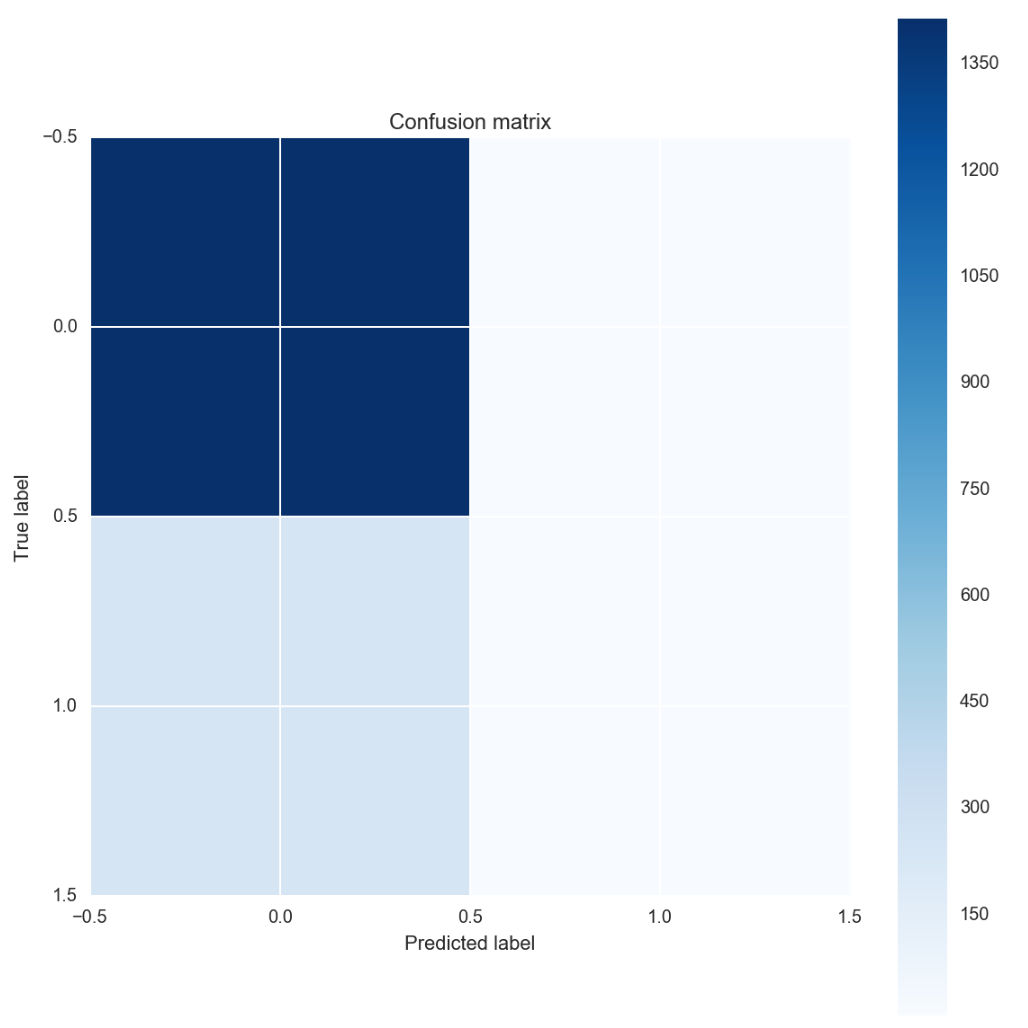
\includegraphics[scale=0.30]{knncm.png} 
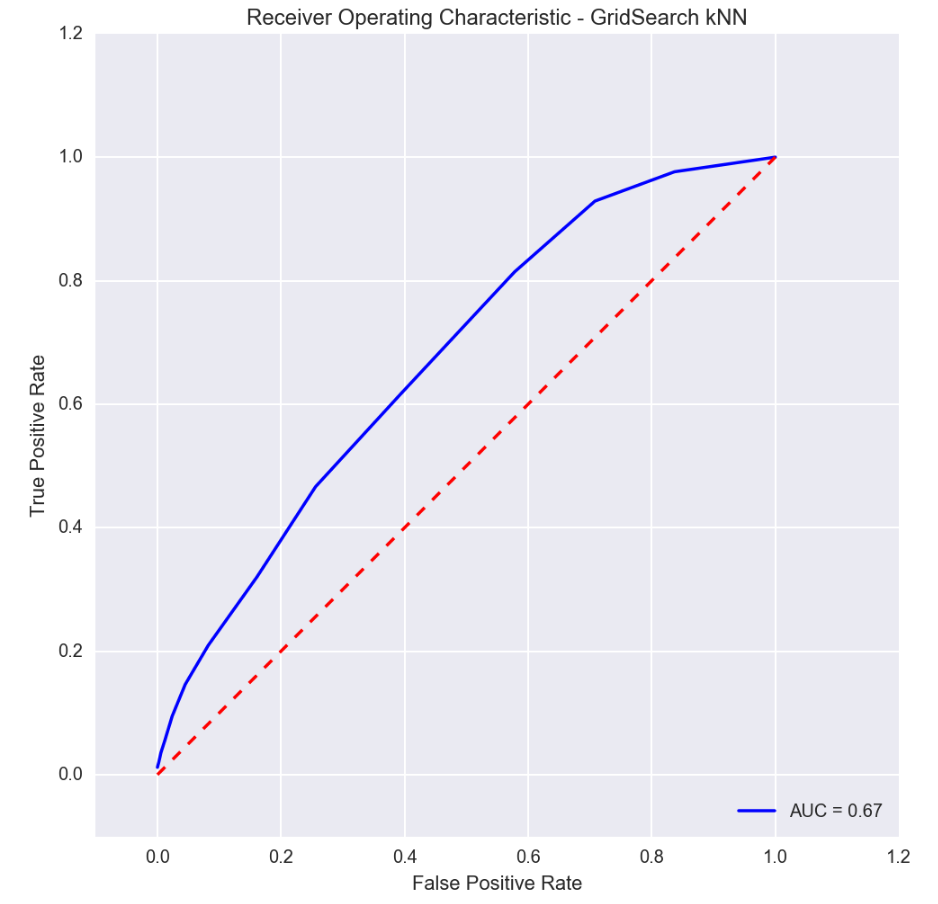
\includegraphics[scale=0.50]{knnroc.png}
\\ \\
The main concern here with kNN is the output seen in the confusion matrix. My precision score was really low at 0.04. In other words, this model only predicted 9 future super hosts out of a sample size of 253.
\\ \\
\indent \indent
The next model I ran was a logistic regression with an l1 penalty (Lasso) because few features were used. This ran better compared to the kNN model with scores:
%ADD SCREEN SHOTS HERE!!!!----------------------------------------------
\\ \\
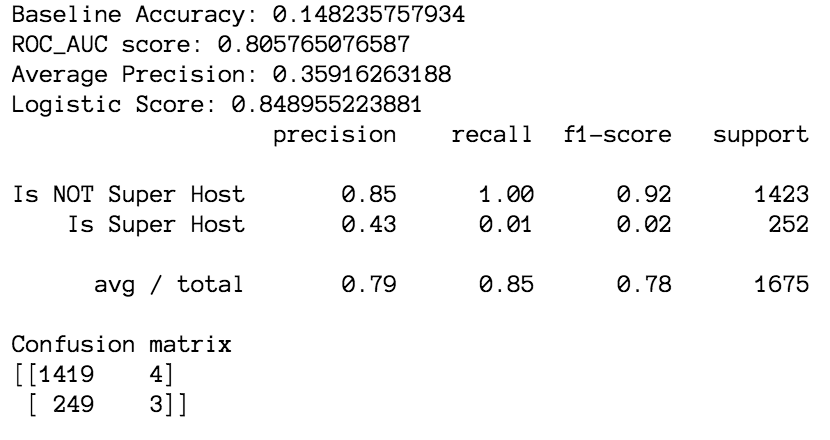
\includegraphics[scale=0.65]{logisticscores.png} \\
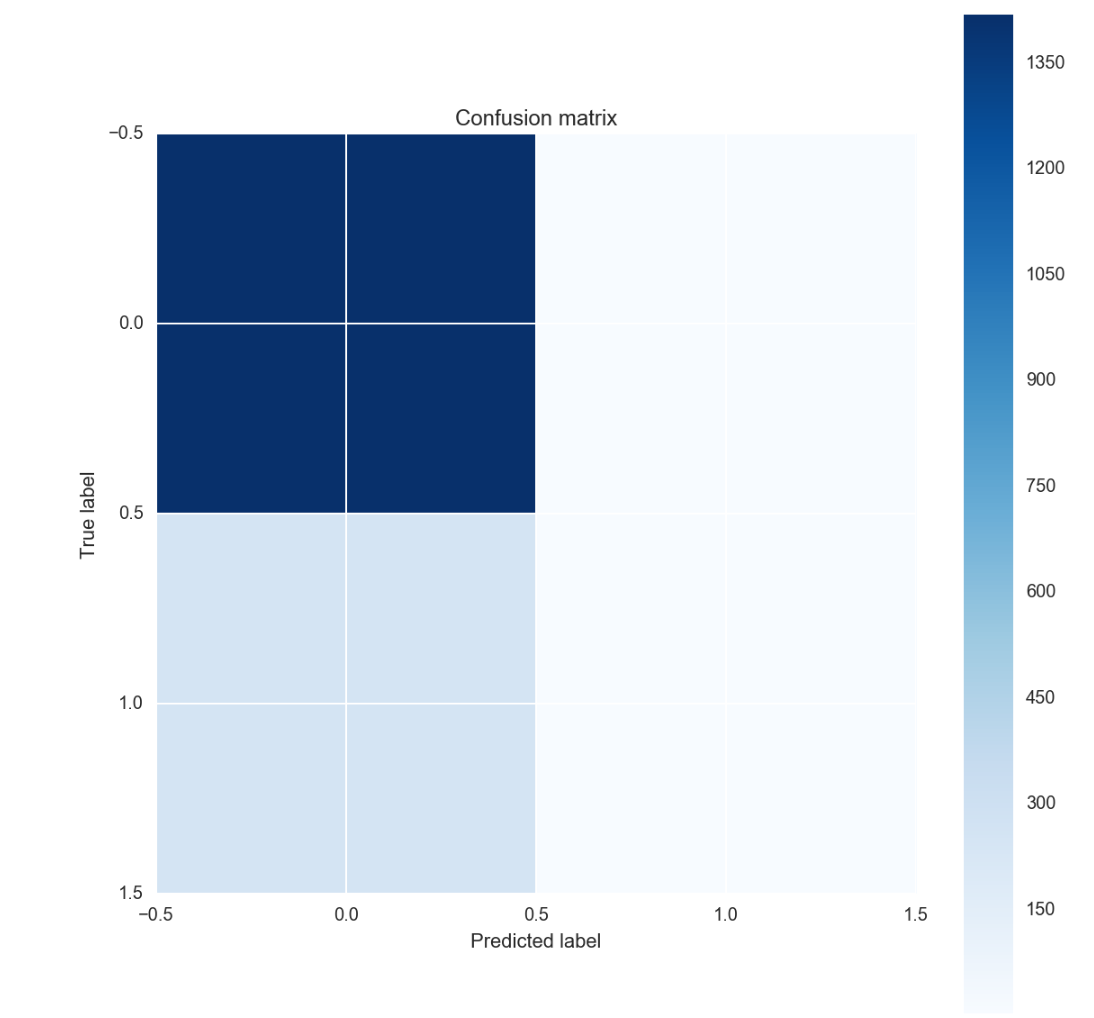
\includegraphics[scale=0.30]{logisticcm.png} 
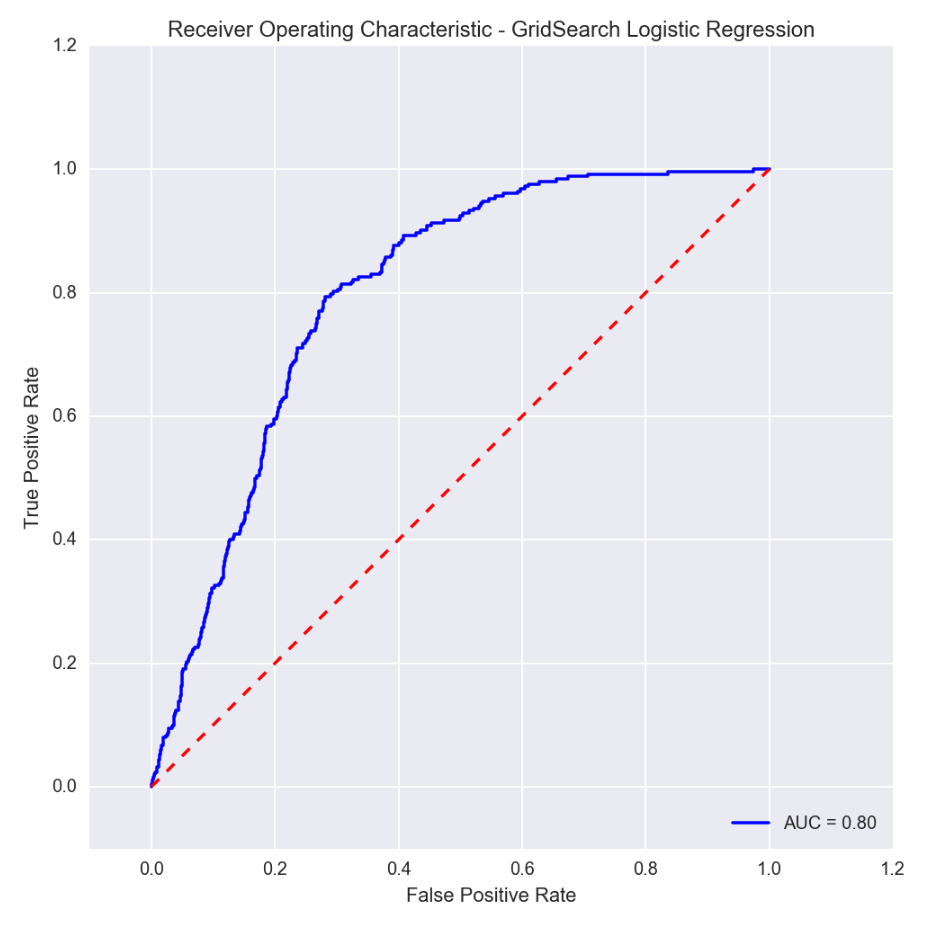
\includegraphics[scale=0.50]{logisticroc.png}
\\ \\
What was great about this model was a ROC score of 0.80 versus kNN's score of 0.67. However, this only predicted a total of 3 super hosts.
\\ \\
\indent \indent Lastly, I performed a Decision Tree Classifier. This came out to be my best model with:
%ADD SCREEN SHOTS HERE----------------------------------------------
\\ \\
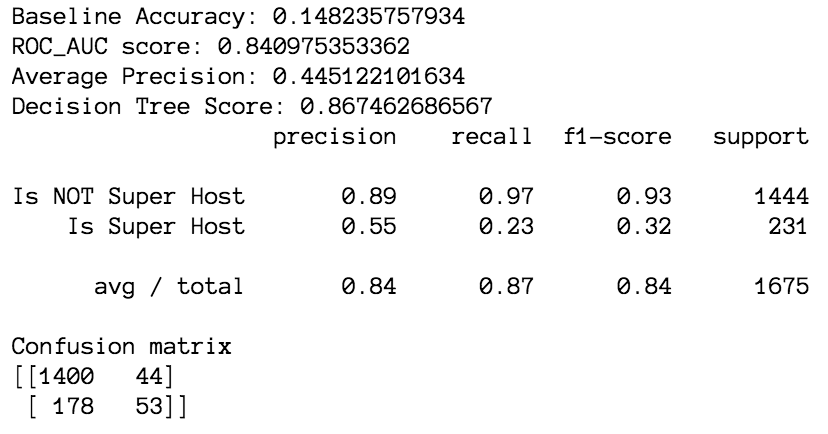
\includegraphics[scale=0.65]{dtcscores.png} \\
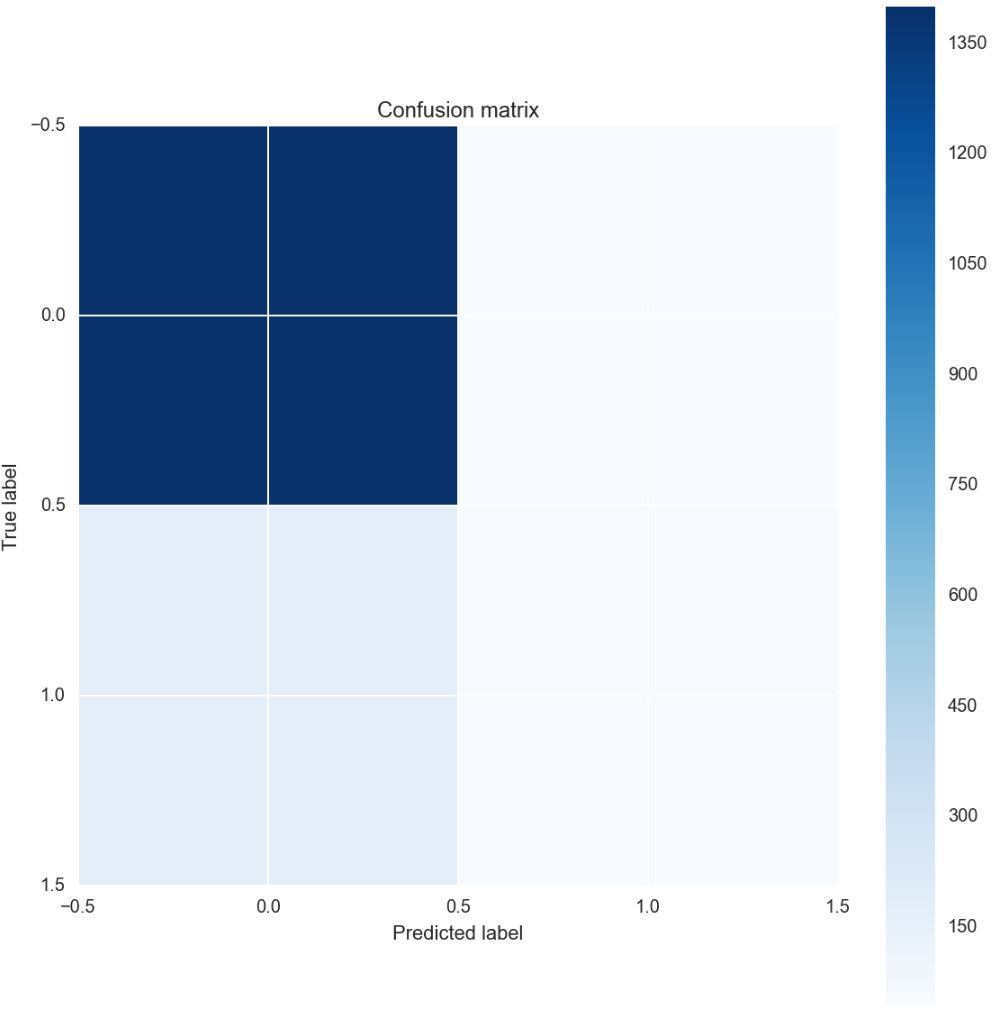
\includegraphics[scale=0.30]{dtccm.png} 
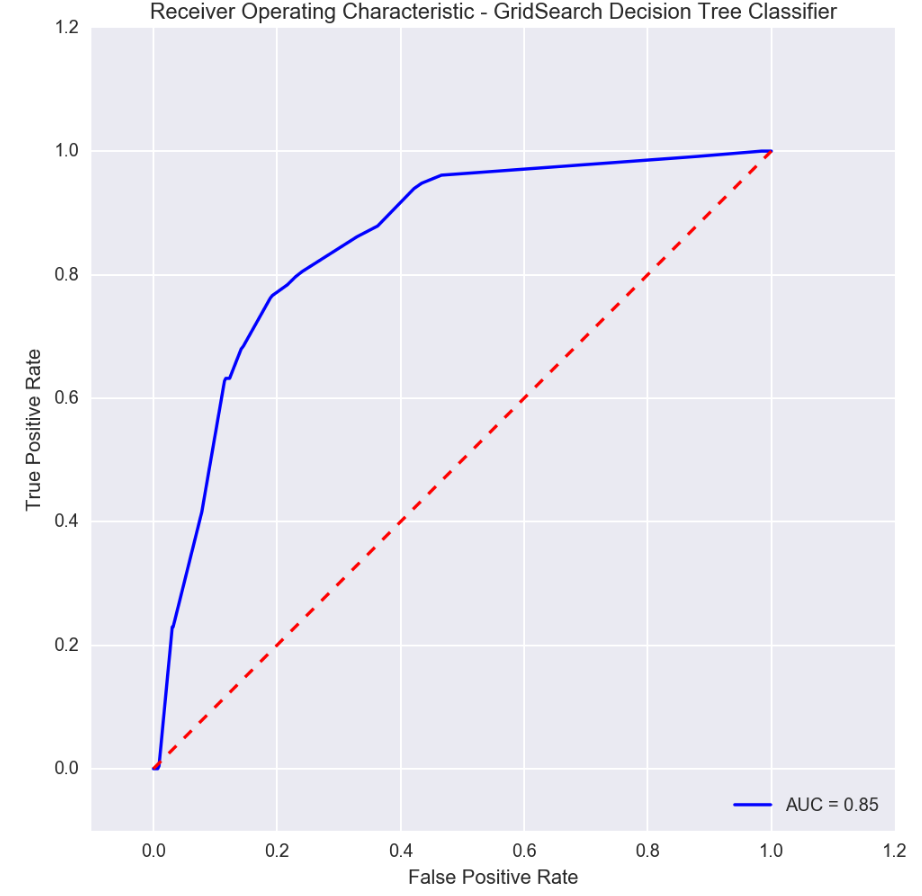
\includegraphics[scale=0.50]{dtcroc.png}
\\ 
The ROC score came out to an astounding 0.85 (85\%) predicting 53 super hosts. Compared to the previous two models, these scores are most impressive. 

\end{paragraph}

%ANALYSIS---------------------------------------------------
\section{Analysis / Conclusion}
\indent 
\indent
\indent
Predicting the amount of super hosts benefits Airbnb's business. Airbnb's revenue comes solely from guests, \textbf{not} hosts. There is a service fee of 3\% charged on hosts. The collection of these fees covers the processing payments between hosts and guests (e.g. Paypal, Visa, MasterCard, etc.). Now, for the guests, there is a 6\% to 12\% fee depending on the listing size. If the reservation was a low price, the fee would be closer to 12\% and if the reservation was a high price, then it would be closer to 6\%. 
\\

\indent \indent
So, what makes a super host so special? One attribute that is most important in this case, is there must be at \textbf{minimum} of 10 reservations. Regardless if the data does not contain bookings, we can assume that every 723 super hosts claimed, has generated 10 times the guests service fees (6\% - 12\%). For example, Sam is a super host who has a listing at \$1,690.00 in the Mission District. For one listing alone, Sam earns \$1,639.30, the guests are charged \$1,791.40, and Airbnb collects \$101.40. However, since Sam is a super host, Airbnb earns at minimum \$1,014.00 (10 bookings times Airbnb's share). This is why super hosts are important for Airbnb's business. In  general, hosts are the liquid assets for Airbnb. No hosts equals no guests which results in no profit. 
\\ \\
\indent \indent 
In conclusion, my hypothesis showed great value for building up more super hosts. However, before doing any research and experimentation, the features or attributes to becoming a super host were different from my theory. Overall, Airbnb's revenue in 2009 totaled to almost \$1 million, now they are projected to hit \$900 million by the end of 2016.

%END OF DOCUMENT--------------------------------
\end{document}

















